\documentclass[11pt,onecolumn]{article}
\usepackage{makeidx,times,alltt,graphicx,calc,subfigure}
\usepackage{xspace}
\usepackage{longtable}
\usepackage{wrapfig}
\usepackage{fancyvrb}
\usepackage{booktabs}
\usepackage{ctable}
\usepackage{multirow}
\usepackage{bigdelim}

\usepackage{epsfig,alltt}
\usepackage{graphics}
\usepackage{shortvrb}
%\usepackage[english,ruled,vlined]{algorithm2e}
%\usepackage{latexsym}
%\usepackage{amssymb,amsmath}
%\usepackage[usenames]{color}
\usepackage{setspace}
\usepackage{comment}
%\usepackage{ulem}

\usepackage{listings}

%\usepackage{pdftricks}
%\begin{psinputs}
%\usepackage{pstricks}
%\usepackage{color}
%\usepackage{pstcol}
%\usepackage{pst-plot}
%\usepackage{pst-tree}
%\usepackage{pst-eps}
%\usepackage{multido}
%\usepackage{pst-node}
%\usepackage{pst-eps}
%\end{psinputs}

%\newcommand{\comment}[1]{}
\newcommand{\charmpp}{\textsc{Charm++}}
\newcommand{\namd}{\textsc{namd}}
\newcommand{\charisma}{Charisma}
\newcommand{\divcon}{\emph{DivCon}}
\newcommand{\openatom}{\textsc{OpenAtom}}
\newcommand{\LeanCP}{\textsc{OpenAtom}}
\newcommand{\leancp}{\textsc{OpenAtom}}
\newcommand{\changa}{ChaNGa}
\newcommand{\kale}{Kale}
\newcommand{\sdag}{Structured Dagger}
\newcommand{\parfum}{{\sc ParFUM}}
\newcommand{\metis}{{\sc Metis}}
\newcommand{\note}[1]{\emph{(Note: #1)}}
\newcommand{\tight}{\baselineskip=8pt}
\newcommand{\etal}{{\em et al.}}
\newcommand{\viz}{{\em viz.}}
\newcommand{\nbody}{$N$-body}
\newcommand{\kdtree}{$k$d-tree}

\def\code#1{{\small {\tt {#1}}}}
\def\smallfbox#1{{\small {\fbox{#1}}}}
\def\porder#1#2#3{$#1 <_{#3} #2$}
\def\lhs#1#2{$#2 \in \mathit{LHS}(#1)$}
\def\rhs#1#2{$#2 \in \mathit{RHS}(#1)$}


\oddsidemargin=-0.25in
\textwidth=7in
\topmargin=-0.25in
\headheight=0in
\headsep=0in
\textheight=9.5in

\begin{document}
%\doublespacing

\title{ NAMD GPU Performance Analysis and Tuning}

\author{
  Yanhua Sun, Xin Zhao\\
  University of Illinois at Urbana-Champaign\\
  \{sun51, xinzhao3\}@illinois.edu
}

\date{}
\maketitle

\lstset{
  basicstyle=\ttfamily,
  showstringspaces=false
}

%\begin{tight}
%\bibliographystyle{abbrv}
%\bibliography{group,cited}
%\end{tight}

\section{Introduction}
In this project, the application we are focusing on is NAMD.
NAMD~\cite{NamdSC02}, recipient of a 2002 Gordon Bell Award, is a parallel molecular 
dynamics code designed for high-performance simulation of large biomolecular systems.
It was developed in the mid-1990's. Now it is one of the most widely used molecular dynamics 
software with more than 50,000 users. It was also selected by NSF as an acceptance test
for Blue Waters.
Through many years, NAMD has been highly optimized to achieve scalable performance on CPU.
It has successfully scaled to the full Titan supercomputer with around $300K$ cores and 
the full Blue Waters with $400K$ cores. In the last 7 years, NAMD has been accommodated
to take the advantage of accelerators, mainly meaning GPGPU. However, it still needs a lot of 
efforts to maximize the performance on GPU. In this project, we are aiming at both 
improve single GPU performance  and scalability on large number of cores. 
%\namd{}

\section{Background}
In a molecular dynamics simulation, a collection of atoms interact through a set of forces. 
Since each atom interacts with all the other atoms, the complexity of calculating forces
is $O(Atoms^2)$. This algorithm does not scale with the number of atoms. Based on the fact that
atoms from far distance contribute little to the force calculation, in \namd{} the interaction is
calculated by short range forces and long range forces. The molecule  is spatially divided into 
patches based on cutoff distance. Atoms in one patch only interact with other atoms in neighbor patches.
To be more accurate, long range electrostatics calculation is performed through particle-mesh Ewald (PME) method.
For these two types of calculation, short range forces are computation intensive while PME is communication intensive.
Therefore, in current NAMD GPU design and implementation, non-bonded cutoff computation is offload to GPU.
All other bonded work, integration and PME work is remained on CPU.

\section{Objective}
After a lot of efforts on optimizing NAMD GPU performance~\cite{phillips_stone_namd_cuda}, NAMD has achieved 
about 10X speed comparing with using one processor-core. However, there is still great
potential space for performance improvement, including tuning on Kepler Tesla K20X and
also improving GPU scalability.

Figures~\ref{figs:apoa1-gpu-singlenode-JYC} and~\ref{figs:apoa1-gpu-scale-JYC}
plot NAMD GPU performance of running the $92K$ atom Apoa1 on a CrayXE/XK machine.
Figure~\ref{figs:apoa1-gpu-singlenode-JYC} shows the performance of running on 
single node with 1 GPU and different numbers of CPU cores. We noticed that increasing
the number of CPU cores actually improves the overall performance up to 5X. Especially, 
using 2 CPU cores provides 2X speedup than using 1 CPU cores.
This is an indication of performance being limited by CPU cores. Furthermore, 
it can be caused by load imbalance between CPU and GPU. In our project, we will profile
and analyze the reason. Hopefully, we will implement a better scheme to balance CPU and GPU load.

Figure~\ref{figs:apoa1-gpu-scale-JYC} illustrates the scalability of 
running Apoa1 simulation on different number of nodes with different configurations of 
(1) GPU with 16 CPU cores(XK7 node), (2) 16 CPU cores only and (3) 32 CPU cores(XE6 node) per node.
On one node, we achieved speed of $3.7x$ and $1.8x$ using GPU, comparing with only using 16 CPU cores
and using 32 CPU cores. However, the benefit of using GPU diminishes with the number of nodes.
Even only on 8 nodes, using GPU does not provide us any improvement compared with using 32 CPU cores.
And the best performance running GPU is only $7.1ms/step$ while it is $2.4$ using 32 CPU cores.
In our project, we will analyze the scaling problem and target at improving GPU scalability.


\begin{figure}[h]
\centering
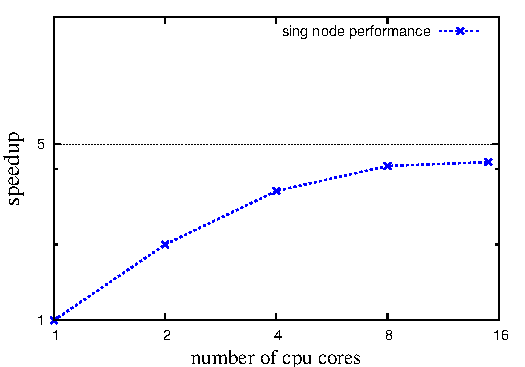
\includegraphics[width=2.8in]{figs/gpu-singlenode}
\caption{Performance of running Apoa1 on one Cray XK7 node using NAMD}
\label{figs:apoa1-gpu-singlenode-JYC}
\vspace{-0.2cm}
\end{figure}

\begin{figure}[h]
\centering
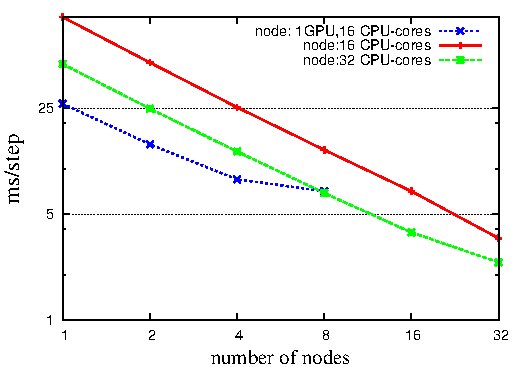
\includegraphics[width=2.8in]{figs/cpu-gpu-jyc-apoa1}
\caption{Scalable performance of running Apoa1 on Cray XK7 and XE6 nodes }
\label{figs:apoa1-gpu-scale-JYC}
\vspace{-0.2cm}
\end{figure}

\section{Milestone}
\begin{enumerate}

\item Profile and analyze single GPU performance of existing implementation to figure 
out the potential performance problem.  We will do more experiments on Kepler GPU. 
\item Try to modify GPU code to solve the above problems
\item Implement scheme to better balance CPU and GPU load 
\item Improve the large-scale running performance

\end{enumerate}

\bibliographystyle{abbrv}
\bibliography{group,cited}
\end{document}


